% Many aspects of this template can be adjusted to
% suit your own preferences. Some parts must remain as they are
% and some parts you should change. Those parts that must remain
% as they are currently are marked with a comment in the LaTeX,
% as are the parts that you should change.

% Keep the font and paper size, but you can change the class and font encoding
% Note: not all classes use \chapter.



\documentclass[a4paper,12pt,oneside]{book}			% sets doc type, book good for chapters
\usepackage[utf8]{inputenc}						% use UTF-8
\usepackage[UKenglish]{babel}						% Ensures proper formatting for English
\usepackage{lmodern}							% Loads latin Modern
\usepackage[LGR,T1]{fontenc}					% LGR = greek letters, T1 = accented Latin letters

% Some common packages, and removal of these will likely break compilation
\usepackage{amsthm,amsmath,amssymb,marvosym} 	% Only really needed if you use maths
\usepackage{graphicx} 							% for including graphics
\usepackage[dvipsnames,svgnames,x11names]{xcolor}	
\usepackage{pdflscape} % for landscape pages
\usepackage{pdfpages} % to insert pages from PDFs


\usepackage[top=2.5cm,						% Define magin spacing
            bottom=2.5cm,
            left=3.2cm,
            right=3.2cm,
            includefoot,
            footskip=30pt,
            ]{geometry}


% \usepackage{lipsum}							used for dummy text i.e. \lipsum[1-3]

% Setting the page layout (headers/footers/etc).
% This can be changed, but ensure that every page of the
% mainmatter is numbered.
\usepackage{fancyhdr}							% Customises headers and footers
\fancyhead[R]{\textsl{\rightmark}}					% Displays current section title in italic in top right
\fancyhead[L]{}								% Leave rop left corner blank
\cfoot{\thepage}								% Place page number in centre of footer
\setlength{\headheight}{15pt}						% Vertical spacing for header

% Adding clickable references and citations
% Also adding PDF metadata and so here you will want
% to change the title and author!
\usepackage[
    pdftex,
    pdftitle={Defensive Honeypot for IoT Devices - Proposal}, 
    pdfauthor={Franek Kruczynski}, 
    pdfkeywords={},
    pdfproducer={LaTeX with hyperref},
    pdfcreator={PDFLaTeX},
    pdfencoding=auto,
    psdextra,
    ]{hyperref}

% Adding the references section (using BibLaTeX).
% Feel free to adjust the style:
%   - ieee (for this style use \cite{name_of_ref})
%   - authoryear (for this style use a combination of \cite{name_of_ref} and \citep{name_of_ref})
\usepackage[
    backend=biber,
    natbib=true,
    style=authoryear,
    ]{biblatex}
\renewcommand\nameyeardelim{, }
\addbibresource{mybib.bib}
\usepackage{csquotes}

% By changing "colorlinks" to true, the boxed link text will
% change the appropriate colour instead of being surrounded
% by a box.
% The colours can be adjusted as you please and there has not
% been much thought put into this colour scheme!
\hypersetup{
    colorlinks=true,
    linkcolor=blue!50!cyan,
    filecolor=magenta,
    urlcolor=blue,
    citecolor=red,
    bookmarksopen=true
    }

% One and half line spacing (this must remain the same)
\linespread{1.25}

% Details to make the title page.
% Change these details!
\title{\huge\bfseries Defensive Honeypots for IP IoT Devices:\\Quantitative  Comparison between Vanilla and Sandboxed Honeypots}
\author{\LARGE Franek Kruczynski}
\date{September 2025}


\begin{document}

\frontmatter			% Uses roman numeral numbering in page number footer
\maketitle				% Creates title from preamble
\setcounter{page}{1}		% reset page counter for contents table
\pagestyle{fancy}

\tableofcontents 			% Creates tableofcontents

\mainmatter 			% Changes page numbering to numbers
\clearpage			




% actual text -----------------------------------
\chapter{Introduction}\label{ch:intro}		% Introduction heading
\section{Background}\label{sec:background}	% Background subheading

The Internet of Things (IoT) is exponentially expanding, with an expected 27 billion devices by the end of 2025 \textit{\citep{autobits2025iot}}. Consequently, this surge resulted in much higher malware sophistication and deployment against IoT devices \textit{\citep{cornell-malware-analysis}}. Such poses a significant risk to IP IoT devices, consumers and infrastructures.

Security researchers and organisations now face rapidly growing challenges in Cyber-attack mitigations. IoT devices often lack robust security measures, use outdated firmware \textit{\citep{security-issue-inIoT}} and vary in network defence levels, leaving them susceptible to malware propagation attacks (its spread).

As a result, malware analysis has become a fundamental practice in Cyber research. Traditional defences like IPS/IDS systems and VPNs often fail against Zero-Day and malicious attacks; while Honeypots (decoy systems mimicking IoT devices) provide effective environment control to attract and analyse attackers \textit{\citep{crowdstrike-honeypot}}.

However, the level of interaction with a Honeypot greatly affects containment and data quality. Low-interaction (vanilla) Honeypots provide easier setup with a constraint on security, whereas high-interaction (sandboxed) Honeypots offer greater analytical processing \textit{\citep{Kocaogullar2023honeypots}}. The balance of containment and interactivity remains a vague area of research. 

This project aims to quantitatively compare sandboxed and vanilla Honeypots, to assess benefits of containment and sandboxing effectiveness in preventing malware mitigation within IoT Honeypot frameworks. 


\section{Aims \&{} Objectives}\label{sec:aimAndObjectives}

\subsection{Aim}\label{sec:aim}

To evaluate the effectiveness of containment and sandboxing mechanisms in preventing malware propagation in IoT Honeypots, through quantitatively comparing identical samples across vanilla and sandboxed Honeypots.

\subsection{Objectives}\label{sec:objectives}
\begin{itemize}

\item Design and deploy a secure Honeynet framework within Virtual Machines (VMs).
\item Deploy two separate Honeypots:
\begin{description}
\item[1.] \textbf{Vanilla Honeypot:} Low-interaction with no advanced security,
\item[2.] \textbf{Sandboxed Honeypot:} High-interaction within a secured container.
\end{description}
\item Create a virtual network with logical addressing and sub-netting for all IoT IP devices and VMs to mimic a small office network.
\item Collect malware properties regarding network traffic, payloads, sample type, activity data and external propagation attempts.
\item Quantitatively compare the data to conclude whether attack behaviours differ based on environment. 
\end{itemize} 


\section{Product Review}\label{sec:productReview}

\subsection{Scope}\label{sec:scope}

The project involves development of a secure IoT Honeynet environment, simulating a small office network composed of two Honeypots, executed sequentially within a singular Lab VM. A separate Analysis VM will store and process sample data using \textbf{ElasticSearch} to guarantee full isolation from external networks.

Each malware sample will be executed within the Honeypots under identical conditions, where the collected data will be stored securely, aiming to reveal the impact of containment.

In essence, findings will lead to a greater understanding regarding the importance of containment. It’ll aid in IoT security through identifying attacker patterns \textit{\citep{Kocaogullar2023honeypots}} and help expand existing research into secure Honeypot environments and design.

\subsection{Audience}\label{sec:audience}

The primary audience relates to Cyber Security researchers, network analysts and academic institutions studying digital forensics and malware analysis. Such groups will benefit from access to data, from a quantitative dynamic analysis, to strengthen threat detection -- for security improvement of developing Honeypots.

Furthermore, the framework will also support students and lecturers by providing a secure and safe virtual environment for malware experimentation and research, to demonstrate analytical and ethical practices. 

Lastly, a comprehensive analysis of malware may support IoT administrators seeking to develop intrusion prevention systems (IDS) \textit{\citep{fortinet-IDS}}, through ensuring critical flaws are unable to be exploited based on historical data.


\chapter{Background Review}\label{ch:backgroundReview}

\section{Existing Approaches}\label{sec:existingApproaches}

Research in malware mitigation includes static analysis and sandboxing systems. Static analysis, such as a Windows-based framework \textit{\citep{static-analysis-drawbacks}} was designed to execute malware within a container, focusing on system registery changes based on run-time behaviour. However, this framework lacks advanced IoT device emulation and has scalability issues regarding resource management, permitting exploitation. 


Systematic and dynamic behavioural analysis of common malware samples \textit{\citep{analysis-mitigation-sandbox-evasion}} within a Cuckoo sandbox provided deep insight into malware attacker patterns. Unfortunately, the ransomware \textit{TeslaCrypt} evaded detection until post-execution, masking the true payload. This demonstrates the concern of poor sandboxing measures in Honeypots. 


\section{Related Literature}\label{sec:relatedLiterature}

IoT-targeting malware research focuses on understanding behavioural patterns and defensive techniques. A graph-based analysis \textit{\citep{cornell-malware-analysis}} focused on polymorphic malware utilising unreachable code, improving general malware classification. Yet, the use of only historical data lacked real-time dynamic collection, crucial for IoT systems.

\textit{\citep{analysis-mitigation-sandbox-evasion}} explored analysis within a popular sandbox, revealing modern malware’s ability to supress execution and remain undetected. It further proved containment alone is not sufficient for IoT system security. Therefore, Honeypot environments require a combination of containment and deception to secure systems effectively.

Lastly, \textit{\citep{crowdstrike-honeypot}} highlights the importance of Honeypots within IoT modern architectures, vital for threat intelligence. However, varying integrations across devices remains a vague area of research. 



\chapter{Methodology \&{} Techniques}\label{ch:methods}
\section{Approach}\label{sec:approach}


The project follows an experimental quantitative comparison to evaluate effectiveness of malware containment within IoT architectures to create a controlled testing environment. Two separate VMs will be deployed using \textbf{Ubuntu} (Lubuntu) within \textbf{Oracle VirtualBox}:
\begin{itemize}
\item\textbf{Vanilla Honeypot}: \textbf{Cowrie} instance operating without additional containment.
\item\textbf{Sandboxed Honeypot}: Identical \textbf{Cowrie} instance inside a \textbf{FireJail} \& \textbf{Docker} container, reinforced with \textbf{Seccomp}, \textbf{WireShark} and \textbf{AppArmor} to restrict system calls and filter network packets.
\end{itemize}

A separate Analysis VM will collect data, process logs and analyse packets using \textbf{ElasticSearch}, ensuring the VM remains disconnected from external networks. Each sample executed within either Honeypot will run in identical conditions to avoid skew. Metrics like network traffic (pcaps), payload data and program events will be stored securely in CSV files.

Integrity will be enforced via kernel-level kill switches, VM snapshot rollbacks and sub-netting to administer traffic isolation. Lastly, all collected sample data will be compared statistically to determine whether sandboxing truly improves containment security. 


\section{Technologies}\label{sec:technologies}

The project will employ various open-source technologies to support controlled analysis. The core framework will operate within \textbf{Oracle VirtualBox}, chosen for its flexibility in sandbox implementation, snapshot management and inter-VM connectivity. Each VM will operate inside \textbf{Ubuntu}, a lightweight and stable Linux distribution.

The Honeypots will be implemented in \textbf{Cowrie}, an SSH/Telnet Honeypot used for capturing IP-based malware, widely used for its logging capabilities for analysis. The sandboxed Honeypot will be containerised within \textbf{Docker}, providing lightweight low-level system isolation; while \textbf{Firejail} \& \textbf{AppArmor}  will enforce kernel-level security by limiting system calls.

For analysis, \textbf{ElasticSearch} will provide real-time log indexing and storage using the RESTful engine complemented by \textbf{WireShark} for packet capturing. \textbf{Python} scripts will extract sample data and format them into appropriate CSV files for final quantitative comparison.




\section{Version Control \&{} Management}\label{sec:versionControl}

All configurations, documentations and scripts will be maintained in \textbf{GitHub} for transparent project development history, with branching used for different development stages and frequent commits.


Backups will be uploaded to \textbf{Google Drive} for redundancy to ensure data synchronisation. Lastly, sensitive data (malware samples and system configs) will remain within the Analysis VM, to ensure ethical and security compliance.



\chapter{Project Management}\label{ch:project management}
\section{Activities}\label{sec:activities}

Project activities align directly with Section~\ref{sec:objectives}:
\begin{itemize}
	\item\textbf{Management Space:}
		\begin{description}
			\item[(1)] Implement a Linux \textbf{nftables} kill switch (kernel-level) to block all IP traffic if containment fails.
			\item[(2)] Establish a management level framework for network addressing, VM management and, snapshot rollbacks.
		\end{description}

	\item\textbf{Virtual Framework:}
		\begin{description}
			\item[(1)] Deploy the Lab VM running \textbf{Cowrie} for both Honeypots.
			\item[(2)] Configure an Analysis VM isolated from external networks.
			\item[(3)] Configure sub-netting and a demilitarised zone to separate Honeypots from the host OS.
			\end{description}

	\item\textbf{Simulation:}
		\begin{description}
			\item[(1)] Execute both Honeypots on \textbf{Cowrie} within \textbf{Lubuntu}, with the sandboxed Honeypot contained.
			\item[(2)] Simulate a small office network to replicate realistic attack patterns.
			\item[(3)] Execute malware samples under strict controlled conditions.
		\end{description}

	\item\textbf{Data Analysis:}
		\begin{description}
			\item[(1)] Capture sample payloads, types and logs.
			\item[(2)] Use \textbf{ElasticSearch} and \textbf{Python} to process data and format into CSV.
			\item[(3)] Conduct quantitative comparison on sample data, analysing relationships across environments.
		\end{description}

\end{itemize}



\section{Schedule and Time Management}\label{sec:time management}
The project will follow a weekly schedule for continuous development:
\begin{itemize}
\item\textbf{Supervisor Meetings:} Weekly meetings for formative feedback.
\item\textbf{Calendar Planning:} Personal calendar to dedicate slots for all aspects of development.
\item\textbf{Time Management:} Personal study will be allocated in daily chunks to balance coursework with dissertation.
\end{itemize}
Finally, a Gantt chart will aid to visualise milestones, with VM snapshot rollbacks integrated into the timeline to avoid test errors. 



\section{Data Management}\label{sec:data management}

All sensitive data (pcaps, logs and samples) will remain within the isolated Analysis VM. Relevant documentation will remain accessible through \textbf{GitHub}. 

Key policies:
\begin{itemize}
	\item\textbf{Ethical Compliance:} No raw sample will leave the contained Honeypots.
	\item\textbf{Backups:} Frequent backups to \textbf{GitHub} and \textbf{Google Drive} to ensure synchronisation. 
	\item\textbf{Isolation:} Strict VM isolation from external networks.
	\item\textbf{Storage:} Process data stored in CSV files for formatted analysis.
\end{itemize}



\section{Deliverables}\label{sec: deliverables}

The project will deliver a secure IoT Honeypot framework with secure sandboxing and a virtual network. The isolated environment will be capable of analysing executed samples.

Additionally, a quantitative dataset containing malware payloads, traffic activity and various logs will be delivered, indexed by \textbf{ElasticSearch}. A comprehensive version-controlled repository will house all scripts, documentation and code.

Lastly, a final analytical report evaluating the effectiveness between malware propagation in Honeypot environments.

In essence, the project aims to deliver a practical research tool and verifiable evidence regarding the effectiveness of containment in IoT Honeypots.


\printbibliography

\begin{appendix}
\chapter{Ethics Form}\label{ch:ethics}
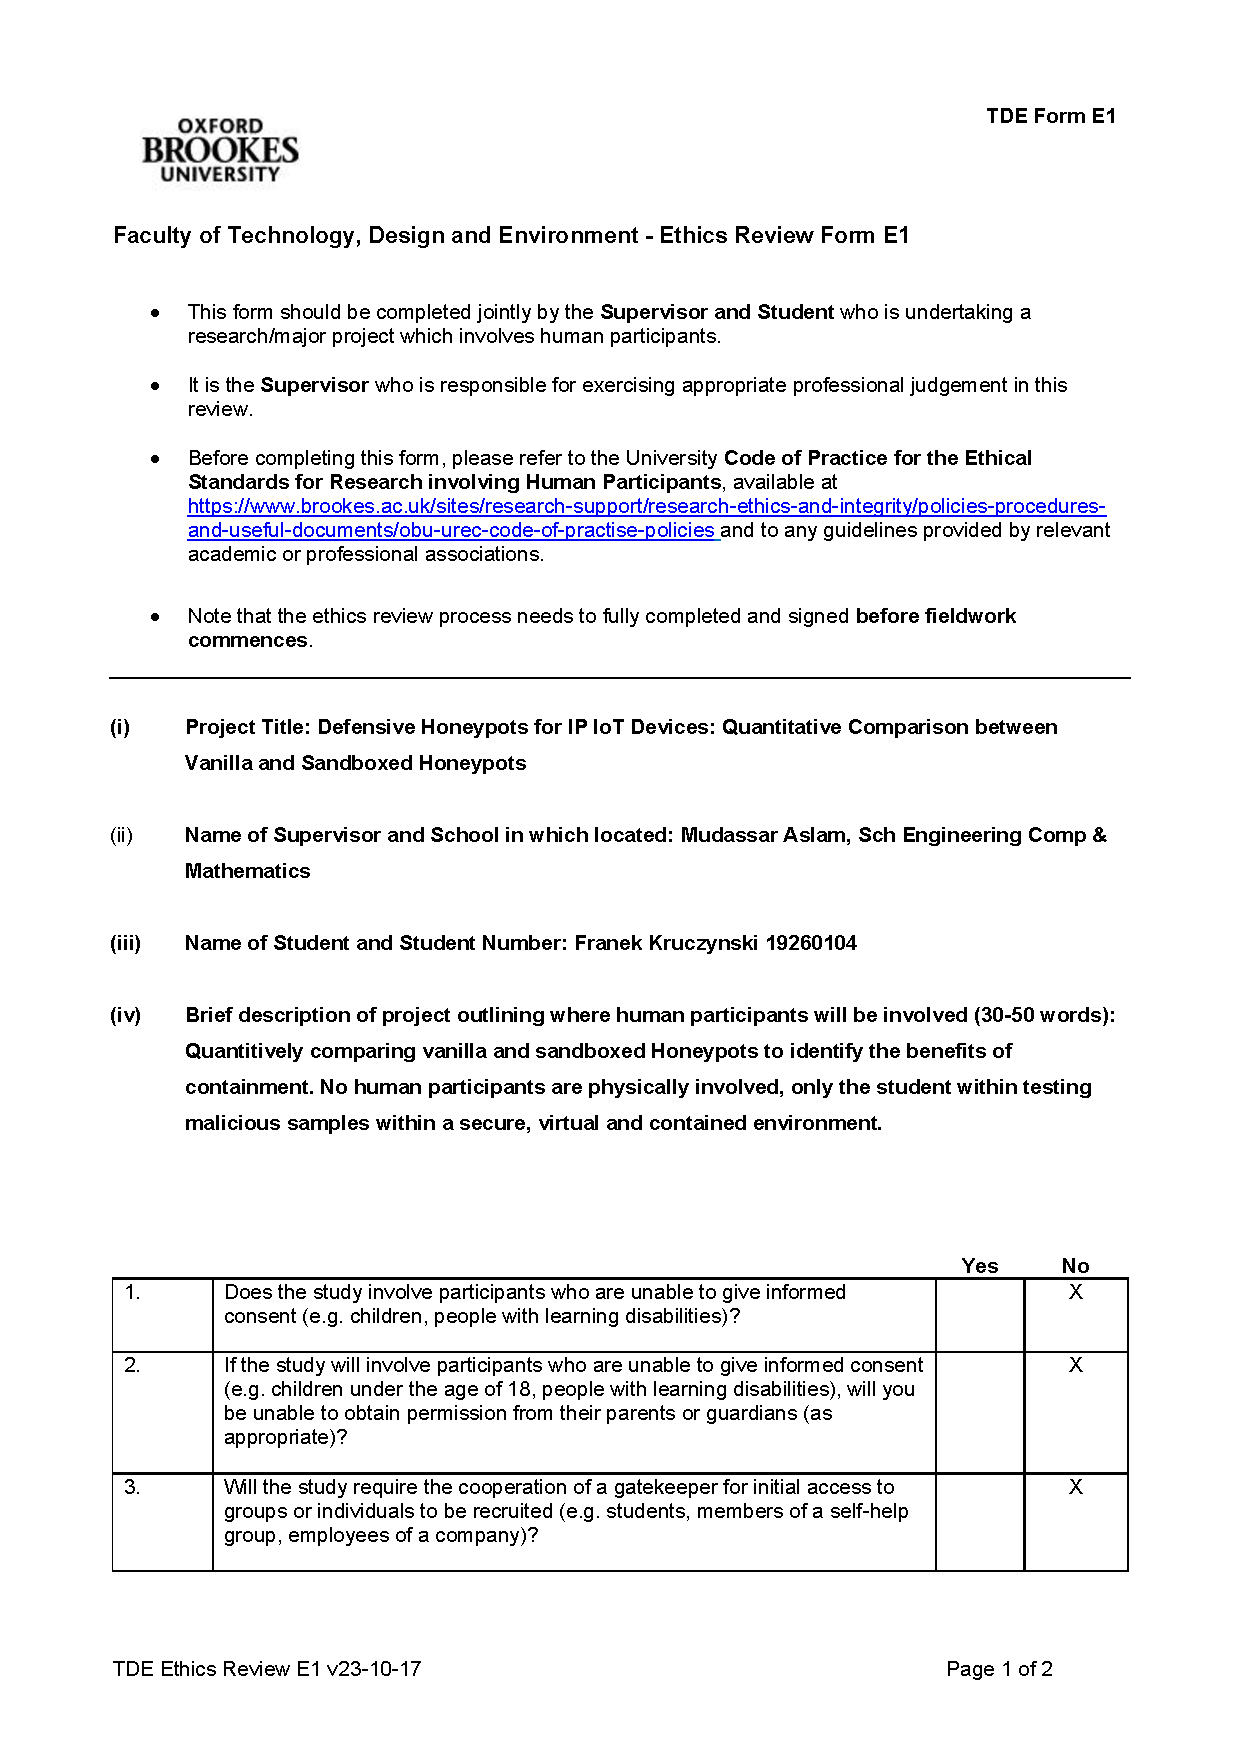
\includepdf[pages=-]{TDE E1 Form.pdf}
\end{appendix}
\end{document}









